\documentclass[10pt]{beamer}
\usetheme[
%%% options passed to the outer theme
%    hidetitle,           % hide the (short) title in the sidebar
%    hideauthor,          % hide the (short) author in the sidebar
%    hideinstitute,       % hide the (short) institute in the bottom of the sidebar
%    shownavsym,          % show the navigation symbols
%    width=2cm,           % width of the sidebar (default is 2 cm)
%    hideothersubsections,% hide all subsections but the subsections in the current section
   hideallsubsections,  % hide all subsections
%    left                % right of left position of sidebar (default is right)
  ]{Aalborg}
  
% If you want to change the colors of the various elements in the theme, edit and uncomment the following lines
% Change the bar and sidebar colors:
%\setbeamercolor{Aalborg}{fg=red!20,bg=red}
%\setbeamercolor{sidebar}{bg=red!20}
% Change the color of the structural elements:
%\setbeamercolor{structure}{fg=red}
% Change the frame title text color:
%\setbeamercolor{frametitle}{fg=blue}
% Change the normal text color background:
%\setbeamercolor{normal text}{bg=gray!10}
% ... and you can of course change a lot more - see the beamer user manual.

\usepackage[utf8]{inputenc}
\usepackage[english]{babel}
\usepackage[T1]{fontenc}
% Or whatever. Note that the encoding and the font should match. If T1
% does not look nice, try deleting the line with the fontenc.
\usepackage{helvet}
\usepackage{setspace}
\usepackage{adjustbox}
\usepackage{graphicx}
\usepackage{bbm}
\usepackage{amsmath}
% colored hyperlinks
\newcommand{\chref}[2]{%
  \href{#1}{{\usebeamercolor[bg]{Aalborg}#2}}%
}
\newcommand\scalemath[2]{\scalebox{#1}{\mbox{\ensuremath{\displaystyle #2}}}}


\title[Finance quantitative]% optional, use only with long paper titles
{Finance quantitative}

\date{\today}

\author[Maksym Bondarenko] % optional, use only with lots of authors
{
Maksym Bondarenko\\
  \href{maksym_bondarenko@outlook.com}{{\tt maksym\char`_bondarenko\char`@outlook.com}}
}
% - Give the names in the same order as they appear in the paper.
% - Use the \inst{?} command only if the authors have different
%   affiliation. See the beamer manual for an example

\institute[
%  {\includegraphics[scale=0.2]{aau_segl}}\\ %insert a company, department or university logo
  CapFi\\
  Paris,France
] % optional - is placed in the bottom of the sidebar on every slide
{% is placed on the bottom of the title page
  CapFi\\  
  Paris, France
  
  %there must be an empty line above this line - otherwise some unwanted space is added between the university and the country (I do not know why;( )
}

% specify the logo in the top right/left of the slide
\pgfdeclareimage[height=1cm]{mainlogo}{AAUgraphics/capfi_logo_baseline_250_250.jpg} % placed in the upper left/right corner
\logo{\pgfuseimage{mainlogo}}

% specify a logo on the titlepage (you can specify additional logos an include them in 
% institute command below
\pgfdeclareimage[height=1.5cm]{titlepagelogo}{AAUgraphics/capfi_logo_baseline_250_250.jpg} % placed on the title page
%\pgfdeclareimage[height=1.5cm]{titlepagelogo2}{AAUgraphics/aau_logo_new} % placed on the title page
\titlegraphic{% is placed on the bottom of the title page
  \pgfuseimage{titlepagelogo}
%  \hspace{1cm}\pgfuseimage{titlepagelogo2}
}

\begin{document}
% the titlepage
{\aauwavesbg
\begin{frame}[plain,noframenumbering] % the plain option removes the sidebar and header from the title page
  \titlepage
\end{frame}}
%%%%%%%%%%%%%%%%

% TOC
\begin{frame}[allowframebreaks]{Contents}{}
\tableofcontents
\end{frame}
%%%%%%%%%%%%%%%%

\section{Introduction}

\subsection{Bases de pricing}

% motivation for creating this theme
\begin{frame}{Qu'est-ce que c'est le pricing?}{}
\begin{block}{}
  \begin{itemize}
    \item Le processus où le business définit le prix d'un produit à vendre \\~\\
    \item Types de produits à valoriser: Options, Futures, Obligations(Business) et Actions (Business) \\~\\
    \item Avant tout on s'intérésse au pricing d'options\\~\\
    \item Types d'options à pricer: Européennes, Americaines, Asiatiques, Exotiques, Binaires etc. 
    
  \end{itemize}
\end{block}
\end{frame}
%%%%%%%%%%%%%%%%

\subsection{Techniques de pricing}

\begin{frame}{Techniques de pricing}{}
\begin{block}{}

    Le but de pricing - trouver le prix "juste" d'un produit financier dont sous-jacent évolue selon certain modèle (théorie). Il existe plusieurs méthodes pour éffectuer le calcul: \\~\\
  \begin{itemize}
    \item Analytique: solution d'une EDP (equation en dérivées partielles) à la main - ne convient pas pour la plupart de types d'options \\~\\
    
    \item Numerique: Solution d'une EDP avec la méthode de differences finies (rapide pour les problèmes avec le petit nombre de sous-jacents, manque de précision)  \\~\\
    
    \item Numerique: Méthodes Monte-Carlo (simulation de scenarios) conviennent pour les problèmes multidimensionels ou si EDP ne peut pas être obtenu
    
  \end{itemize}
\end{block}
\end{frame}
%%%%%%%%%%%%%%%%

\begin{frame}{L'example de pricing}{}
\begin{block}{}
    
   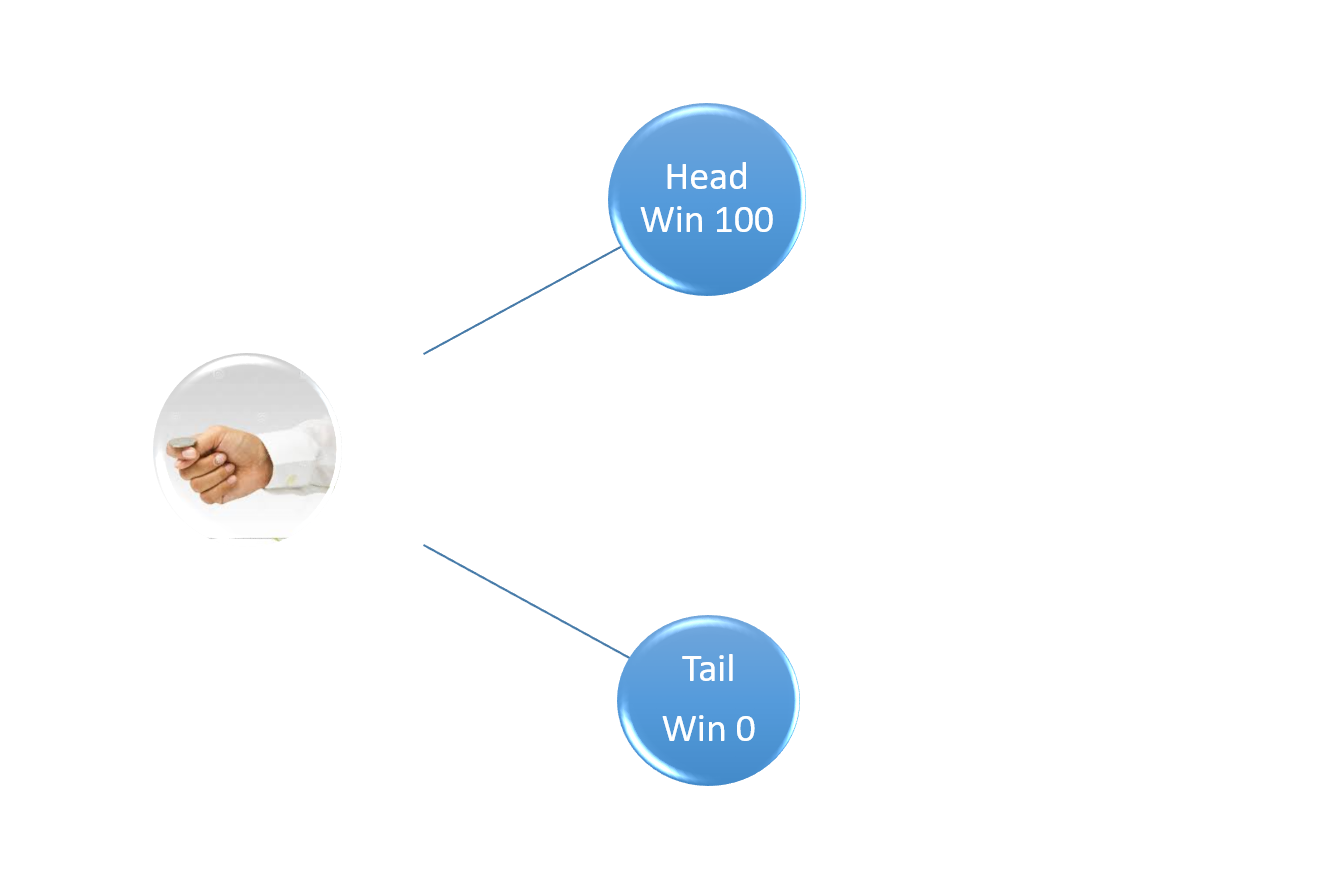
\includegraphics[width=8cm]{AAUgraphics/example1.png}
   
   \begin{itemize}
        \item Combien auriez-vous payé pour ce jeu? Si vous avez 200? Si vous avez 1000?
   \end{itemize}
    
\end{block}
\end{frame}
%%%%%%%%%%%%%%%%

\begin{frame}{L'example de pricing}{}
\begin{block}{}

\scriptsize{  \begin{itemize}
        \item Si vous avez pas assez de capital pour jouer plusieurs fois, vous accepterez de payer le prix au dessus ou en dessous de l'esperance en fonction de votre appetit pour le risque \\~\\
        \item Dans le logique risque neutre (1000 Euro) $ E_{win} = 100*proba_{win} + 0*proba_{lose} = 100*0.5 + 0*0.5 = 50 $ \\~\\
        \item Dans le logique risque prenneur (200 Euro) $ E_{win} = 100*proba_{win} + 0*proba_{lose} = 100*0.7 + 0*0.3 = 70 $  \\~\\ 
        \item Dans le logique risque averse (200 Euro) $ E_{win} = 100*proba_{win} + 0*proba_{lose} = 100*0.3 + 0*0.7 = 30 $  \\~\\
        \item On appelle l'ensemble de probabilités ($proba_{win}$, $proba_{loss}$) la \textbf{mesure risque neutre} (l'estimation de probas par investisseur comme s'il était indifférent par rapport au risque) \\~\\
        
        \item Si on vous propose ce genre de jeu au casino ou bien sur le marché d'options sachez que le prix de produit sera définit selon la mesure risque neutre. Cette mesure est déduite de prix de produits simples et réutilisée ensuite pour valoriser les produits plus complexes
        
   \end{itemize}
    
    }
\end{block}
\end{frame}
%%%%%%%%%%%%%%%%

\subsection{Théorie}

\begin{frame}{La mesure risque neutre et actif sans risque}{}
\begin{block}{}

\scriptsize{  \begin{itemize}
        \item La mesure risque neutre est telle ensemble de probas que le prix d'un actif aujourd'hui (sur le marché) est égale à l'esperance \textbf{actualisé} de ce prix sous cette mesure \\~\\
        
        \item Une autre façon d'en penser: telle ensemble de probas sous laquelle tous les actifs ont le même taux de rendement (taux sans risk) \\~\\
        
        \item L'actif sans risque (dont le prix est 100 si le taux égale à zero):
        
        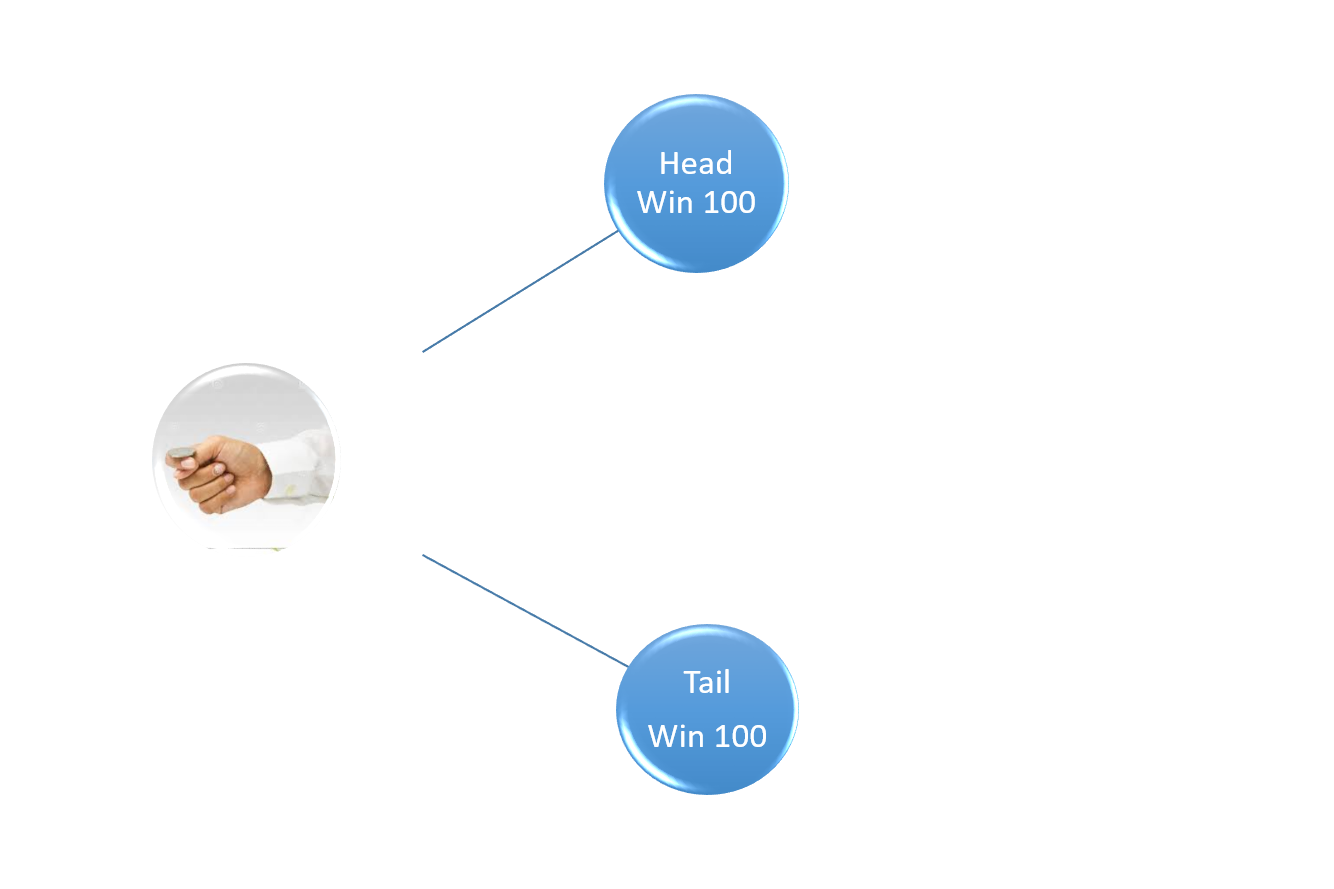
\includegraphics[width=8cm,height=4cm,keepaspectratio]{AAUgraphics/riskfree.png}
        
   \end{itemize}
    
    }
\end{block}
\end{frame}
%%%%%%%%%%%%%%%%


\begin{frame}{La mesure risque neutre et actif sans risque}{}
\begin{block}{}

\scriptsize{  \begin{itemize}
        \item Theoreme fondamentale du pricing\\~\\
        Le marché est AOA (absence d'opportunité d'arbitrage) seulement s'il existe une mesure risque-neutre \\~\\
        Autrement dit: il existe une mesure sous laquelle tous les process de prix sont martingales (esperance de rendement actualisé demain est égale au prix aujourd'hui) \\~\\
        
 \item Algorithme: \\~\\
 Trouver une mesure risque-neutre en utilisant le modèle de dynamique de prix du sous-jacent \\~\\ 
 Utiliser cette mesure pour trouver les prix des produits derivés sur ce sous-jacent
        
        
   \end{itemize}
    
    }
\end{block}
\end{frame}
%%%%%%%%%%%%%%%%











\section{Mono-periode}



\subsection{Marché de deux actifs}


\begin{frame}{Option européenne}{}
  \begin{itemize}
    \item Option européene est un produit financier (contrat) qui donne a son teneur droit et pas l'obligation d'acheter ou vendre l'actif sous-jecent pour le prix prédéfinit à la date d'écheance prédéfinite\\~\\
  \end{itemize}
  \begin{figure}[!tbp]
  \centering
  
    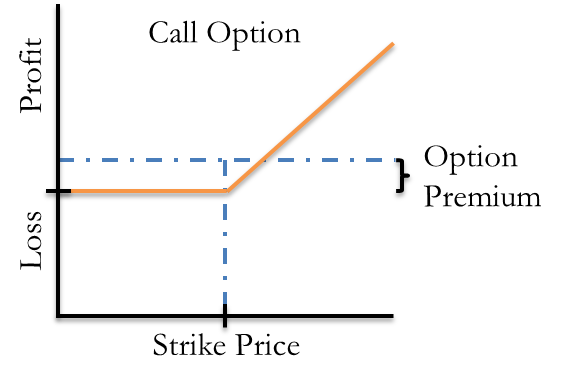
\includegraphics[width=8cm,height=8cm,keepaspectratio]{AAUgraphics/call.png}
   
\end{figure}
  
\end{frame}
%%%%%%%%%%%%%%%%



% the license
\begin{frame}{Marché de deux actifs}{}
  \begin{itemize}
    \item Imaginons qu'on a un actif sans risque et un actif risqué qui coutent 100 Euros aujourd'hui\\~\\
  \end{itemize}
  \begin{figure}[!tbp]
  \centering
  \begin{minipage}[b]{0.4\textwidth}
    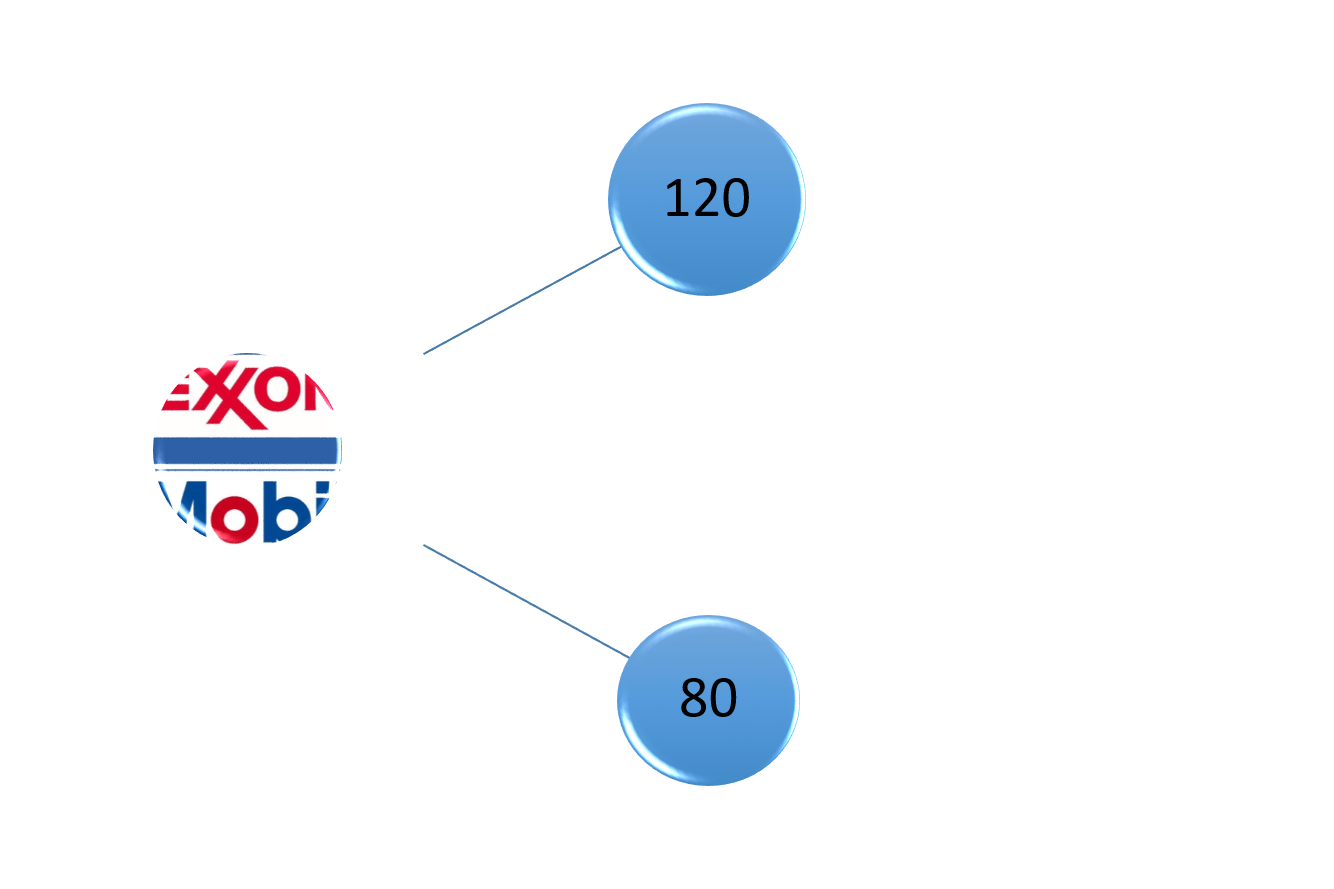
\includegraphics[width=8cm,height=3cm,keepaspectratio]{AAUgraphics/Picture2.png}
    \caption{actif risqué}
  \end{minipage}
  \hfill
  \begin{minipage}[b]{0.4\textwidth}
    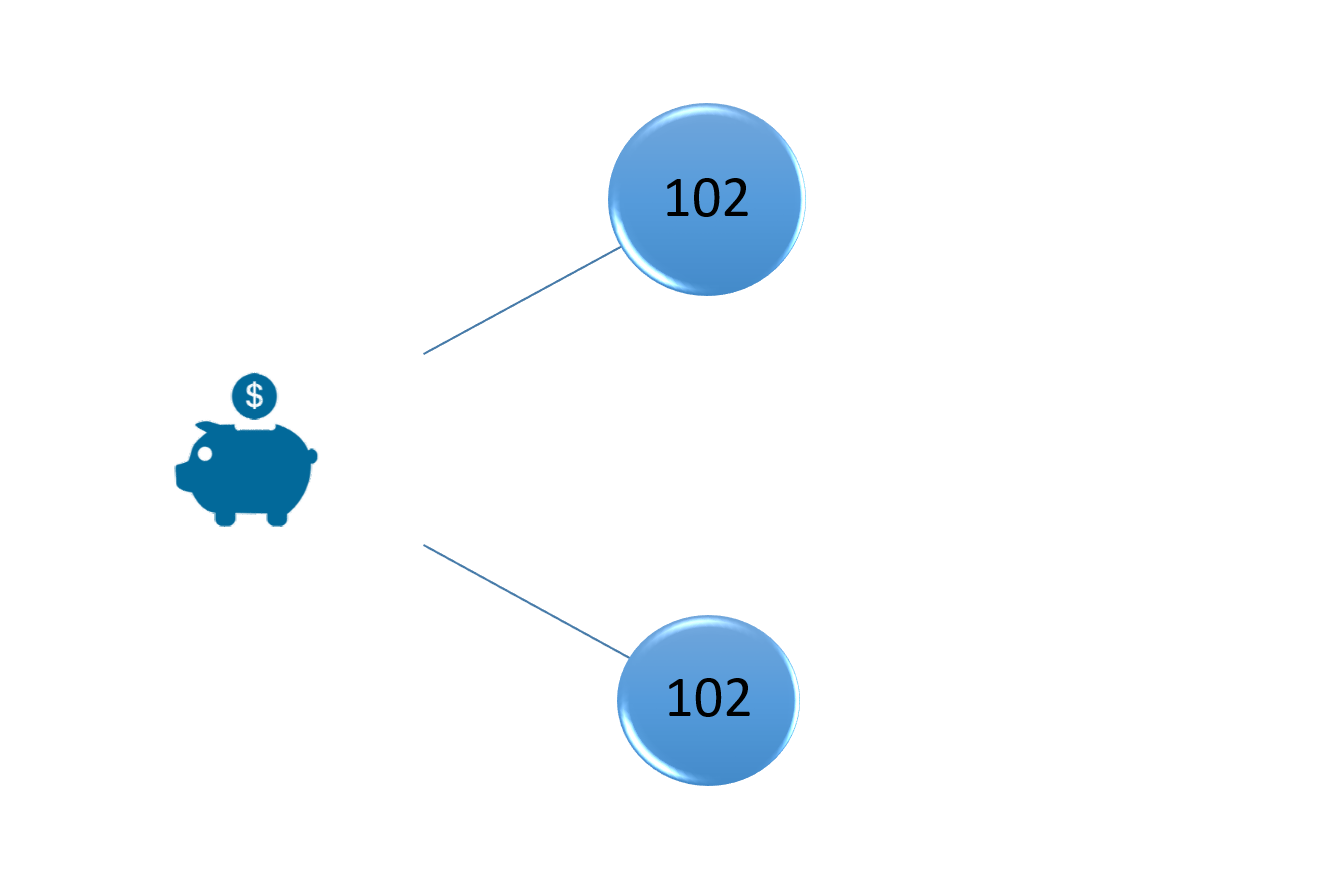
\includegraphics[width=8cm,height=3cm,keepaspectratio]{AAUgraphics/Picture3.png}
    \caption{actif sans risque}
  \end{minipage}
\end{figure}

\small{
Notre but: trouver le prix d'une option européenne dont le sous-jacent est Exxon mobil. L'option nous donne le droit d'acheter une action Exxon pour 100 Euro. Taux sans risque est égale à 2\% 
}
  
\end{frame}
%%%%%%%%%%%%%%%%



\begin{frame}{Marché de deux actifs: comment pricer?}{}
\small{
    \begin{enumerate}
      \item Trouver la mesure risque neutre
      \begin{math}
       
        \left\{
        \begin{array}{r c l}

            \frac{120*q_{1} + 80*q_{2}}{1+r} = 100 \\~\\ 

            \frac{102*q_{1} + 102*q_{2}}{1+r} = 100 \\ 
       \end{array}
       \right\}
      \end{math} \\~\\ \\~\\
  
    On résoud cette équation et on obtient: $q_{1} = \frac{11}{20}$ and $q_{2} = \frac{9}{20}$ \\~\\
  
      \item Trouver le prix de payoff $Option = \frac{(Exxon-K)_{+}}{1+r}$ \\~\\
      
      $E[(Exxon-K)_{+}]_{Q} = \frac{(120-100)_{+}*\frac{11}{20} + (80-100)_{+}*\frac{9}{20}}{1+0.02} = \frac{20*\frac{11}{20}+0}{1.02} = \frac{11}{1.02} = 10.78$
    \end{enumerate}
      
  }
  
  Evidemment si on valorisait l'option avec la mesure $(p_{1} = 0.5, p_{2} = 0.5)$ la valeur obtenu serait moins de 10 alors y a risk-premium sur ce marché
  
\end{frame}
%%%%%%%%%%%%%%%%





\subsection{Marché de troix actifs}
% the license
\begin{frame}{Marché de troix actifs}{}
  \begin{itemize}
    \item Imaginons qu'on a un actif sans risque et deux actifs risqués qui coutent 100 Euros aujourd'hui\\~\\
  \end{itemize}
  
 

\begin{figure}[t]
\centering

\subfigure{
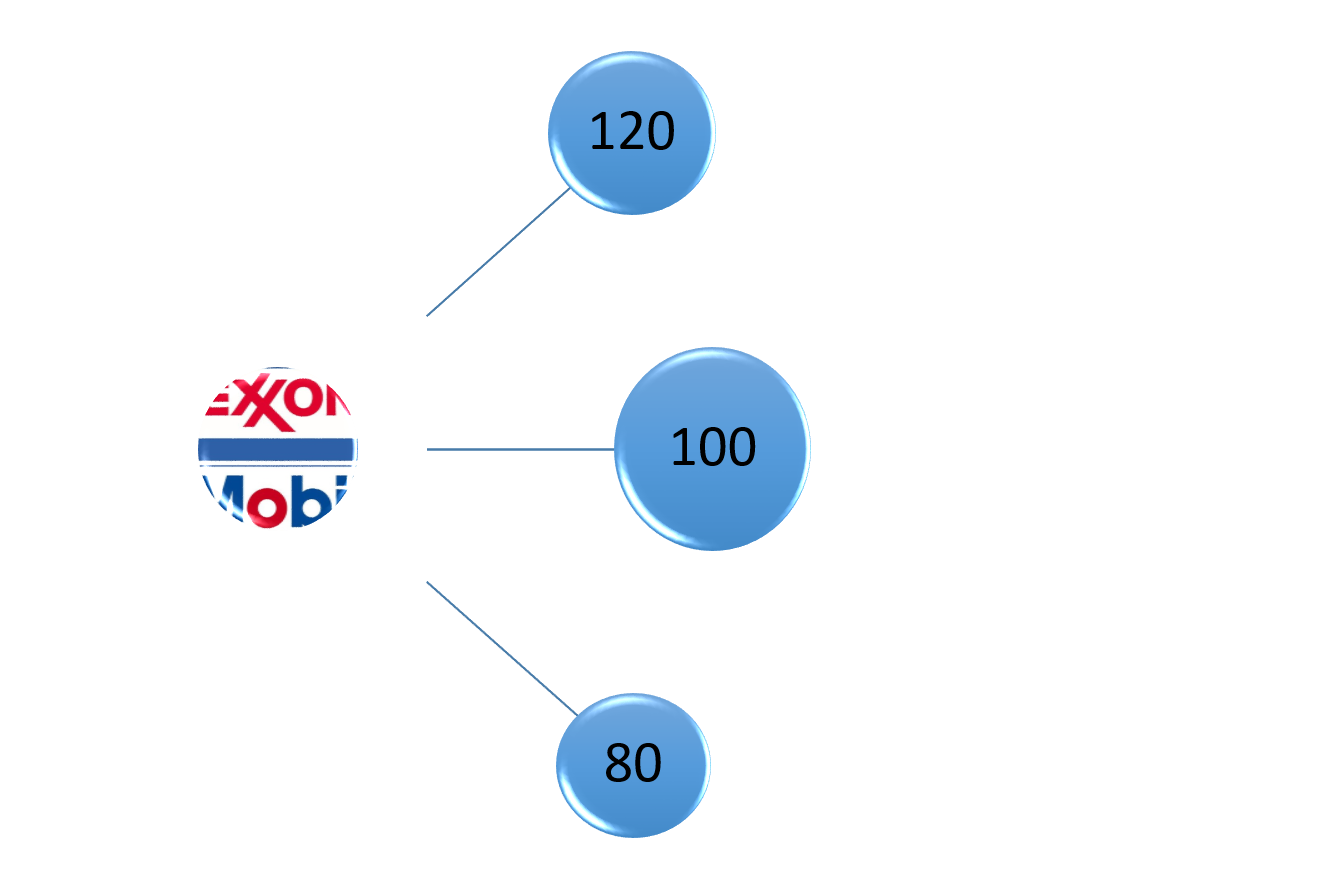
\includegraphics[width=.3\textwidth]{AAUgraphics/Picture5.png}
}

\subfigure{
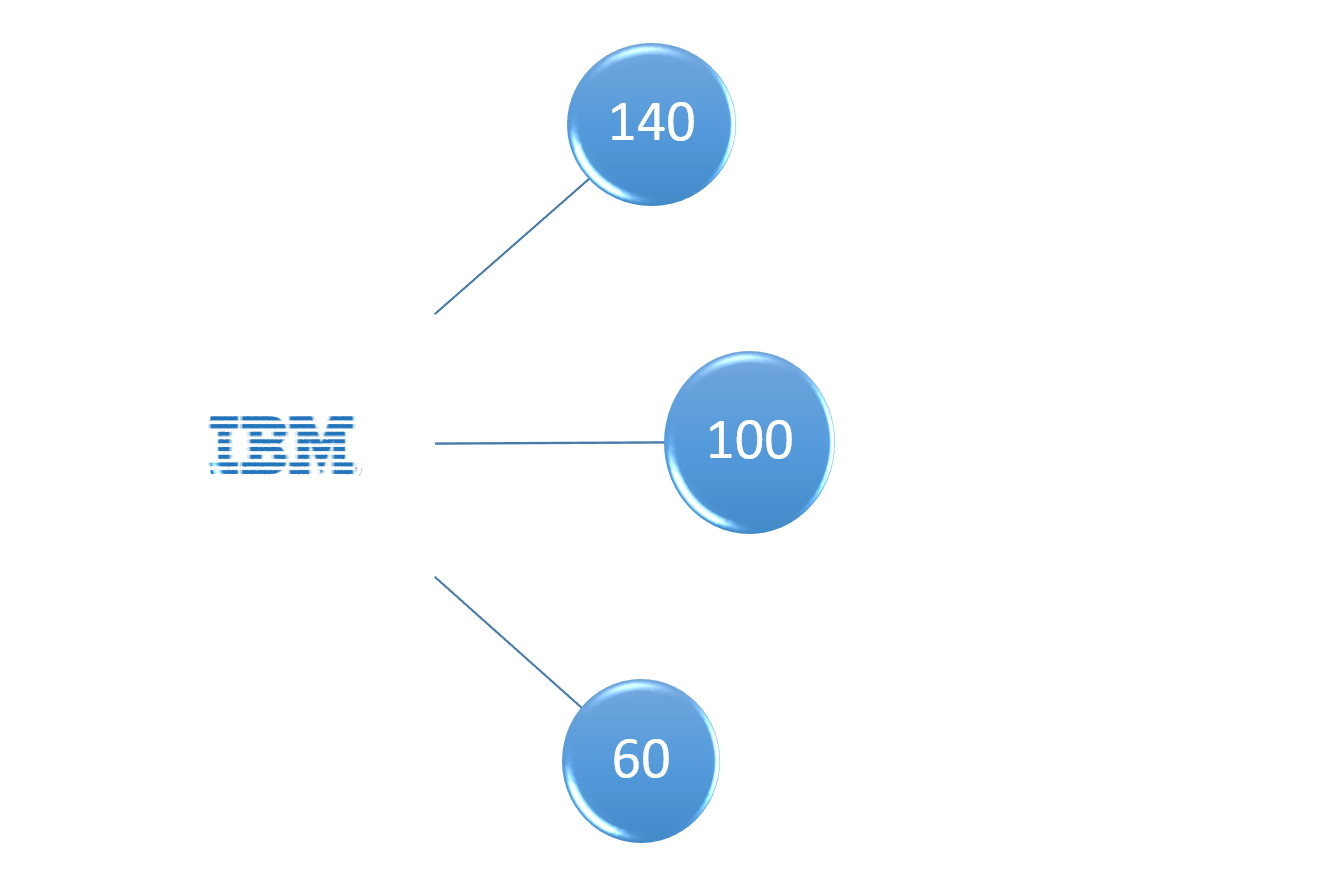
\includegraphics[width=.3\textwidth]{AAUgraphics/Picture4.png}
}

\subfigure{
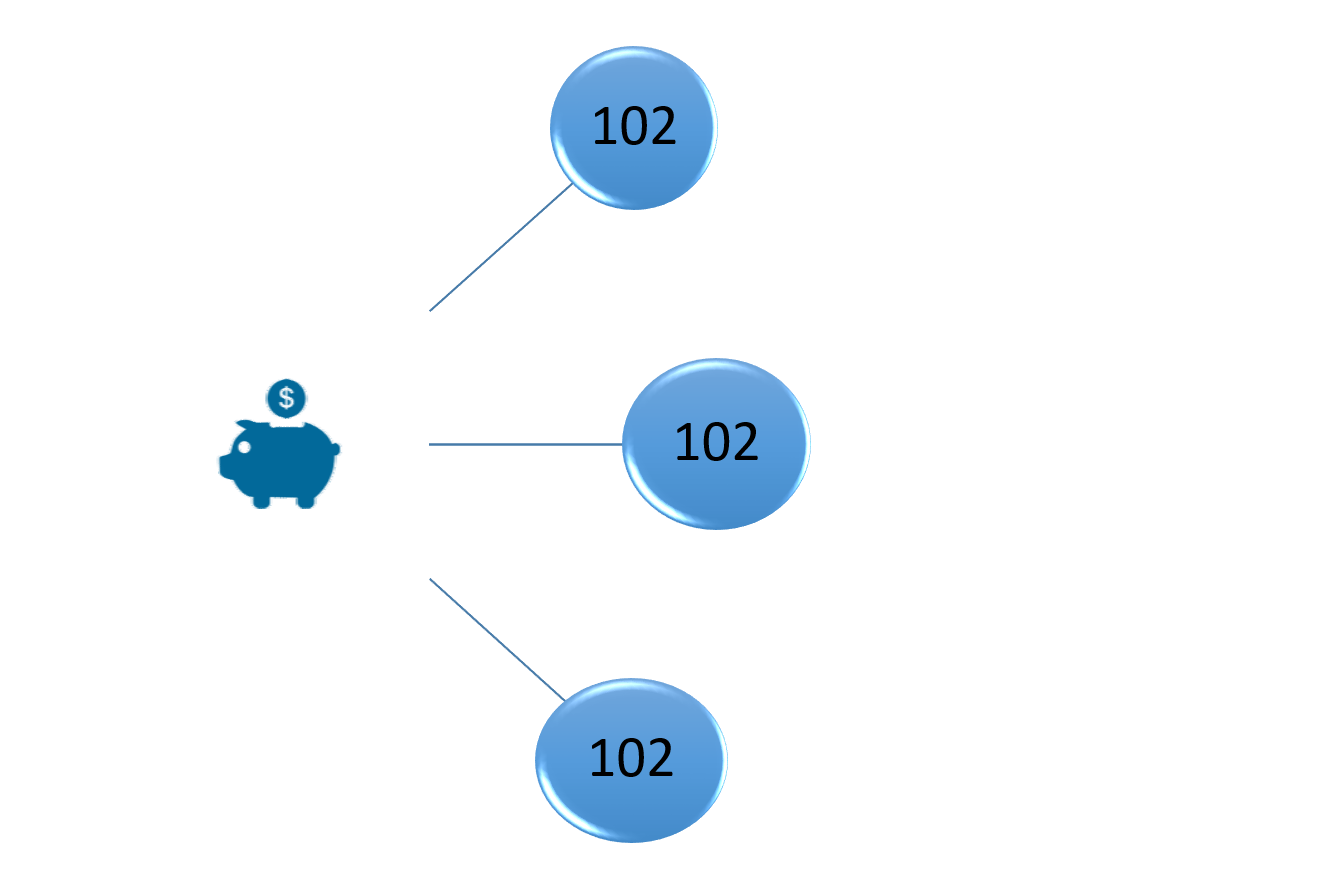
\includegraphics[width=.3\textwidth]{AAUgraphics/Picture6.png}
}
\end{figure}

\end{frame}
%%%%%%%%%%%%%%%%


\begin{frame}{Marché de troix actifs: cas incomplet}{}
\small{
    \begin{enumerate}
      \item Trouver la mesure risque neutre
      \begin{math}
       
        \left\{
        \begin{array}{r c l}

            \frac{120*q_{1} + 100*q_{2} + 80*q_{3}}{1+r} = 100 \\~\\ 
            
            \frac{140*q_{1} + 100*q_{2} + 60*q_{3}}{1+r} = 100 \\~\\ 

            \frac{102*q_{1} + 102*q_{2} 102*q_{3}}{1+r} = 100 \\ 
       \end{array}
       \right\}
      \end{math} \\~\\ \\~\\
  
    On résoud cette équation et on obtient: $q_{1} = \frac{1}{3}$, $q_{2} =\frac{1}{3}$ and $q_{3} = \frac{1}{3}$ \\~\\
    ou une autre combinaison:
    $q_{1} = \frac{1}{4}$, $q_{2} =\frac{1}{4}$ and $q_{3} = \frac{1}{2}$ \\~\\
  
    \end{enumerate}

 }
  
  En effet la mesure n'est pas unique ça veut dire qu'on ne peut pas valoriser un produit derivé d'une manière unique. Le marché ou la mesure risque neutre est unique s'appelle \textbf{marché complet}. Marché est incomplet également dans le cas où il y a 3 actifs et deux états de nature
  
\end{frame}
%%%%%%%%%%%%%%%%



\begin{frame}{Marché de troix actifs: cas complet}{}
  \begin{itemize}
    \item Imaginons qu'on a un actif sans risque et deux actifs risqués qui coutent 100 Euros aujourd'hui\\~\\
  \end{itemize}
  
 

\begin{figure}[t]
\centering

\subfigure{
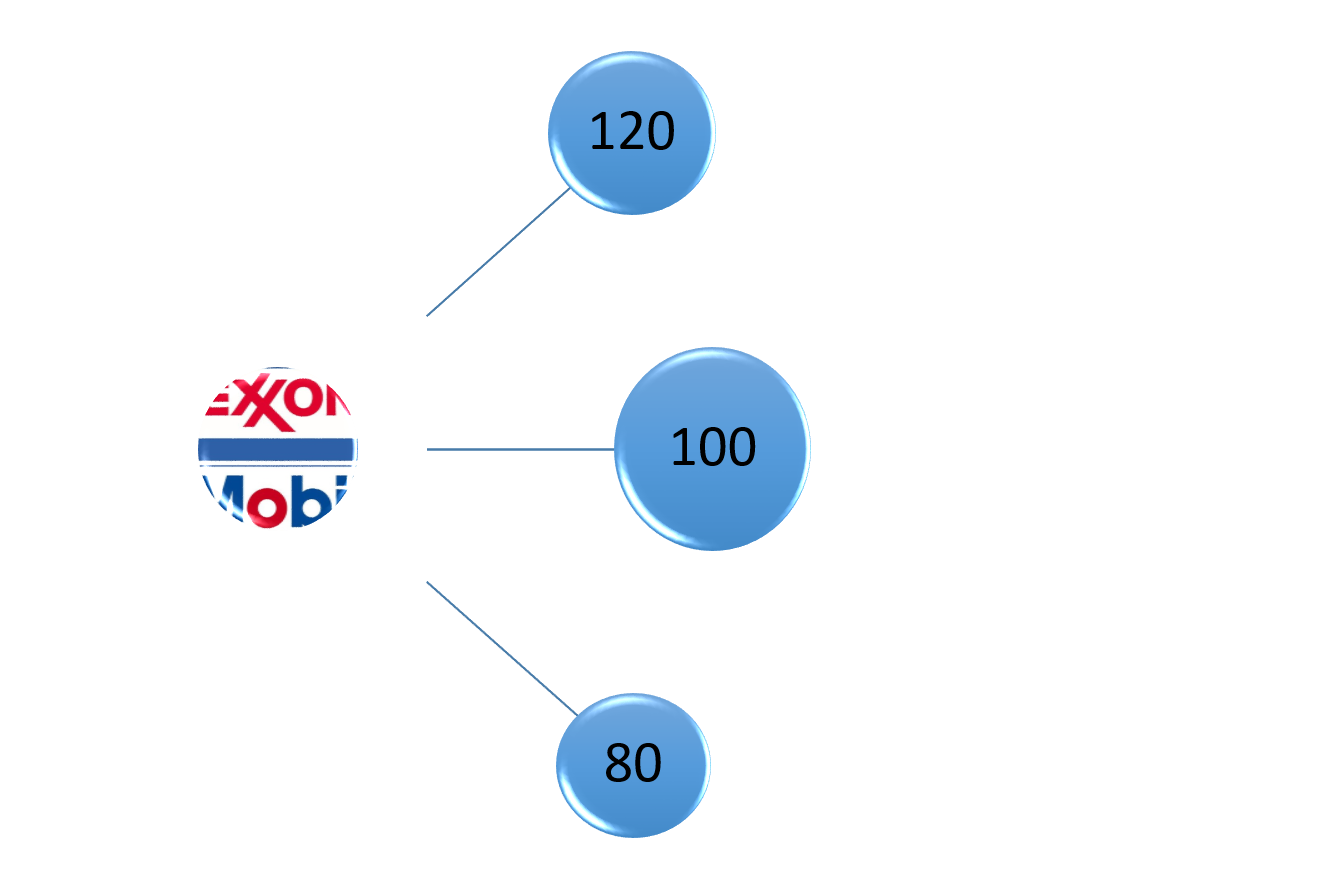
\includegraphics[width=.3\textwidth]{AAUgraphics/Picture5.png}
}

\subfigure{
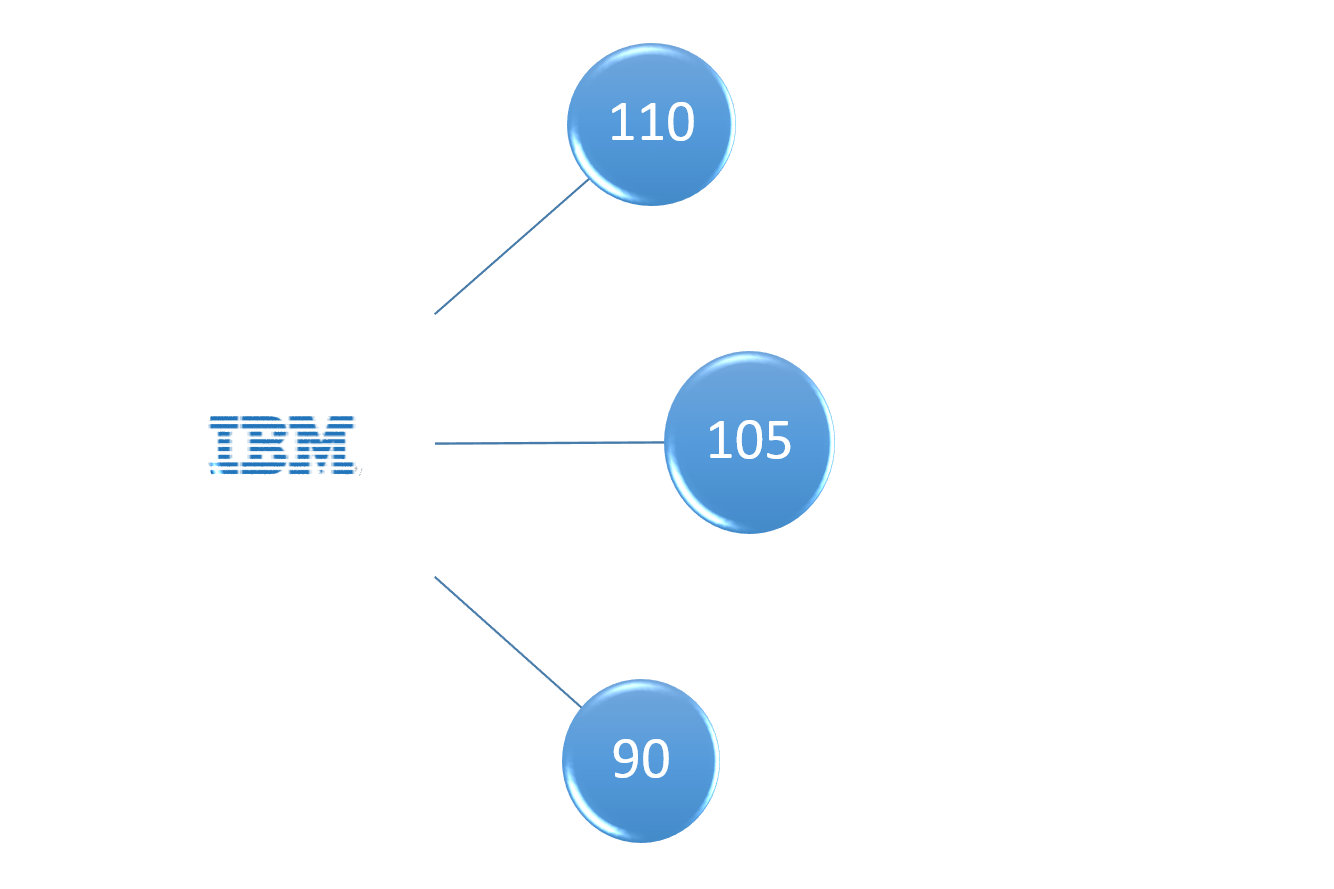
\includegraphics[width=.3\textwidth]{AAUgraphics/Picture7.png}
}

\subfigure{
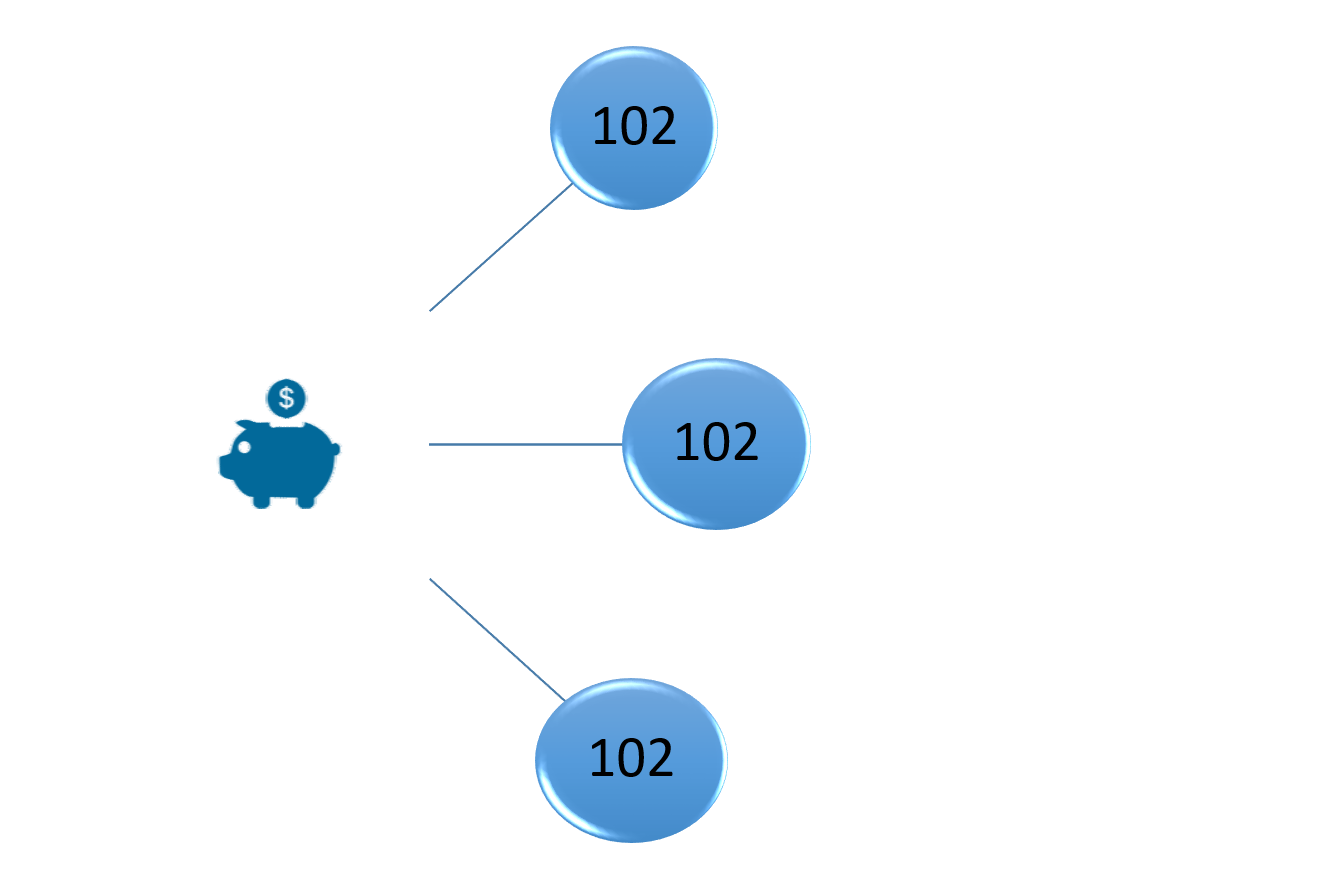
\includegraphics[width=.3\textwidth]{AAUgraphics/Picture6.png}
}
\end{figure}

\end{frame}
%%%%%%%%%%%%%%%%



\begin{frame}{Marché de troix actifs: cas complet}{}
\scriptsize{
    \begin{enumerate}
      \item Trouver la mesure risque neutre \\~\\
      \begin{math}
       
        \left\{
        \begin{array}{r c l}

            \frac{120*q_{1} + 100*q_{2} + 80*q_{3}}{1+r} = 100 \\~\\ 
            
            \frac{110*q_{1} + 105*q_{2} + 90*q_{3}}{1+r} = 100 \\~\\ 

            \frac{102*q_{1} + 102*q_{2} 102*q_{3}}{1+r} = 100 \\ 
       \end{array}
       \right\}
      \end{math} \\~\\ \\~\\
  
    On résoud cette équation et on obtient: $q_{1} = \frac{9}{20}$, $q_{2} =\frac{1}{5}$ and $q_{3} = \frac{7}{20}$ \\~\\
   qui est unique alors on peut valoriser une option
    \end{enumerate}
    
    

 }
 
 Notre but: trouver le prix d'une option européenne dont le deux sous-jacents est Exxon mobil et IBM. L'option nous paie la difference entre moyen prix de Exxon et IBM et le prix strike K = 100 si positif. Taux sans risque est égale à 2\% \\~\\
  
  $Price[Option] = \frac{E[(\frac{Exxon+IBM}{2} - K)_{+}]_{Q}}{1+r}$ \\~\\ $ = \frac{(\frac{120+110}{2}-100)_{+}*\frac{9}{20}+(\frac{105+100}{2}-100)_{+}*\frac{1}{5}+(\frac{80+90}{2}-100)_{+}*\frac{7}{20}}{1.02} = 7.11$
  
\end{frame}
%%%%%%%%%%%%%%%%

\subsection{Hedging}

\begin{frame}{Hedging}{}
\begin{itemize}
\item But \\~\\
 Gagner la prime en tant que vendeur d'une option tout en restant invulnérable aux fluctuations du marché (soient-elles positives ou negatives) \\~\\
 
 \item Strategie de replication \\~\\
 Avoir un portefeuille d'actifs qui replique le prix d'une option à tout moment \\~\\
 \end{itemize}
 
 \end{frame}
 
\begin{frame}{Hedging mono-periode}{}
 $\boldsymbol{X=S\theta} $  ou $X$ - payoff en temps T, $S$ - matrice de prix d'actifs en temps T, $\theta $ - portefeuille de replication
Revenons à notre example:
  $Price[Option] = \frac{E[(\frac{Exxon+IBM}{2} - K)_{+}]_{Q}}{1+r}$ \\~\\ $ = \frac{(\frac{120+110}{2}-100)_{+}*\frac{9}{20}+(\frac{105+100}{2}-100)_{+}*\frac{1}{5}+(\frac{80+90}{2}-100)_{+}*\frac{7}{20}}{1.02} = 7.11$
  
  \begin{gather}
 \begin{bmatrix} 15 \\ 2.5 \\ 0 \end{bmatrix}
 =
  \begin{bmatrix}
   102 &
   120 & 
   110 \\
   102 &
   100 &
   105 \\
   102 & 
   80  &
   90 \\
   \end{bmatrix}
   \begin{bmatrix} \theta_{1}\\ \theta_{2} \\ \theta_{3} \end{bmatrix}
\end{gather} \\~\\
  
  alors hedging portfolio $\theta$ =  \begin{bmatrix}
   \frac{10}{51} \\
   \frac{7}{8} \\
   -1 
   \end{bmatrix} \\~\\
   avec $V(\theta)_{0} = $
   \begin{bmatrix}
   \frac{10}{51} \\
   \frac{7}{8} \\
   -1 
   \end{bmatrix} 
   \begin{bmatrix}
   100 &
   100 &
   100 
   \end{bmatrix} = 7.11
  
 
\end{frame}



\section{Black Scholes framework}


\subsection{Introduction}


\begin{frame}{Pourquoi Black Scholes}{}
  \begin{itemize}
    \item Modélisation en temps continu\\~\\
    \item Marché est complet sous Black Scholes alors on peut toujours valoriser des options\\~\\
    \item Le rendement de sous-jacent suit la distribution normale  $N(r-\frac{\sigma^{2}}{2}, T\sigma)$\\~\\
    \item Les sous-jacents suivent ce modéle  \\~\\
    
    
  \end{itemize}
  
 \begin{figure}[t]
\centering

\subfigure{
 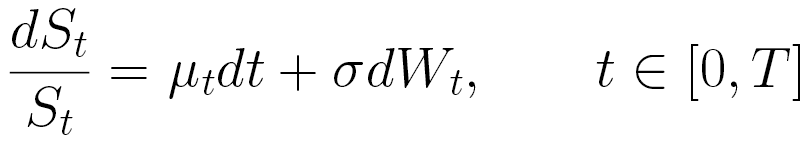
\includegraphics[width=5cm,height=5cm,keepaspectratio]{AAUgraphics/bsmodel.png}
}
%\subfigure{
%\includegraphics[width=5cm,height=5cm,keepaspectratio]{AAUgraphic%s/blackscholes-1.png}
%}

\end{figure}

\end{frame}

\begin{frame}{Derivation de mesure risque-neutre}{}
 \begin{itemize}
    \item Selon les series de Taylor\\~\\
    $dF(S,t) = \frac{dF}{dt}dt +\frac{dF}{dS}dS + \frac{1}{2}\frac{d^{2}F}{dS^{2}}dS^{2}$\\~\\
    \item Remplacons dS \\~\\
     $dF(S,t) = \frac{dF}{dt}dt +\frac{dF}{dS}(\mu Sdt+\sigma SdW_t) + \frac{1}{2}\frac{d^{2}F}{dS^{2}}(\mu ^{2} S^{2}(dt)^{2} + 2\mu \sigma S^{2}d_tdW_t +\sigma ^{2}S^{2}dW_tdW_t)$\\~\\
     \item Regroupons les termes \\~\\
     $dF(S,t) = (\frac{dF}{dt} +\frac{dF}{dS}\mu S + \frac{1}{2}\frac{d^{2}F}{dS^{2}}\sigma ^{2} S^{2})dt + \frac{dF}{dS}\sigma SdW_t$\\~\\
     
 \end{itemize}
\end{frame}

\begin{frame}{Derivation de mesure risque-neutre}{}
 \begin{itemize}
    \item Remplacons $F(S,t)=log(S_t)$  \\~\\
    $log(S_t)-log(S_0) = (\mu - \frac{1}{2}\sigma ^{2})dt + \sigma dW_t$\\~\\
    \item Passons dans un monde risque-neutre  de $\mu$ vers $r$ en utilisant Girsanov $W_{t} = \bar{W_{t}} + \frac{r-\mu}{\sigma}t$ \\~\\
    $S_t = S_0  e ^ {(\mu - \frac{1}{2}\sigma ^{2})t + \sigma W_t} = S_0  e ^ {(r - \frac{1}{2}\sigma ^{2})t + \sigma \bar{W_t}} $\\~\\
    \item Trouvons l'esperance \\~\\
    $E[S_t] = S_0 * E[e ^ {(r - \frac{1}{2}\sigma ^{2})t + \sigma \bar{W_{t}}}] = S_0 e^{rt} E[e ^ {- \frac{1}{2}\sigma ^{2}t + \sigma \bar{W_{t}}}] = S_0 e^{rt}$\\~\\
     
 \end{itemize}
\end{frame}

\subsection{Méthodes Monte Carlo}

\begin{frame}{Pricing avec Monte Carlo: dans quel cas?}{}
  \begin{itemize}
    \item Utilisé s'il n'y a pas de solution exacte (Modéles de volatilité stochastique et locale) \\~\\
    
    \item Utilisé s'il y a plusieurs sous-jacents ou plusieurs sources d'incertitude (plus rapide que les différences finies): Basket, Options Americaines \\~\\
    
  \end{itemize}
  
  \centering
  $S_T = S_0  e ^ {(r - \frac{1}{2}\sigma ^{2})T + \sigma \bar{W_T}} $ avec $W_T = N(0,T)$ \\~\\ 
  
  \begin{figure}[t]
\centering

%\subfigure{
% 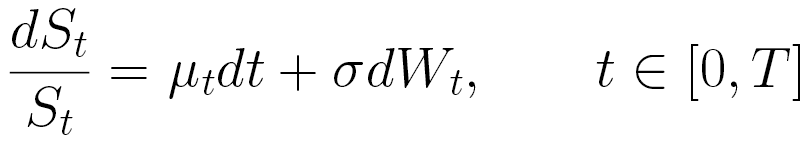
\includegraphics[width=5cm,height=5cm,keepaspectratio]{AAUgraphics/bsmodel.png}
%}

\subfigure{
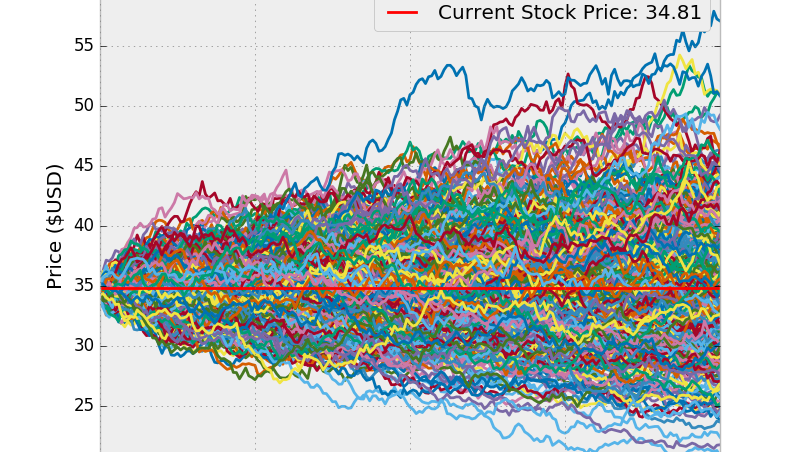
\includegraphics[width=6cm,height=5cm,keepaspectratio]{AAUgraphics/montecarlo.png}
}

\end{figure}


\end{frame}






\begin{frame}{Pricing avec Monte Carlo}{}
  
 \begin{itemize}
    \item Payoff d'une option\\~\\
    $X = (S_T - K)_+$ \\~\\
    \item Prix d'une option sous la mesure risque-neutre avec n - nombre de simulations monte-carlo (n assez grand => par la loi de grands nombres la moyenne arithmetique converge vers l'esperance)\\~\\
    $ P_0 = E[X] = E[(S_T - K)_+] = 
    \frac{\sum\limits_{i=1}^n (S_0 e^{(r - \frac{1}{2}\sigma ^{2})T + \sigma N_i(0,T)} - K)*I_{S_{T_i}>K}}{n} $
    
  \end{itemize}

\end{frame}


\subsection{Calibration}

\begin{frame}{Calibration}{}
  
Dans le monde réel nous ne connaissons ni le prix de l'action demain ni les valeurs $r$ et $\sigma $ \\~\\

La tache de calibration est un problème inverse de pricing et consiste à trouver les paramètres $r$ et $\sigma $ à partir des prix des options existantes sur le marché \\~\\

Dans le modèle de Black-Sholes nous connaissons la soultion exacte de son EPD:\\~\\

 \begin{figure}[t]
\centering

\subfigure{
\includegraphics[width=5cm,height=5cm,keepaspectratio]{AAUgraphics/blackscholes-1.png}
}

\end{figure}

Solution pour un call est: \\~\\
$C = N(d1)S_0 - N(d2)Ke^{-rT}$ \\~\\ avec $d_1 = \frac{ln(\frac{S_0}{K})+(r+\frac{\sigma ^ {2}}{2})T}{\sigma \sqrt{T}}$ et $d_2 = d_1 - \sigma \sqrt{T}$

\end{frame}

\begin{frame}{Calibration}{}

 \begin{figure}[t]
\centering

\subfigure{
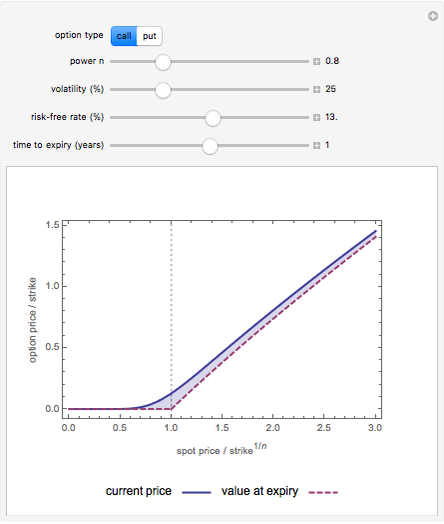
\includegraphics[width=10cm,height=7cm,keepaspectratio]{AAUgraphics/bssurf.png}
}

\end{figure}

\end{frame}

\begin{frame}{Calibration}{}
  La tache de calibration se formalise donc: \\~\\
  $G(\sigma) = \inf(\sum \limits_{i=1}^{x} (C_{market}(T,K)_i - C_{BS}(S,T,K,\sigma , r)_i))$ 
  
  \begin{itemize}
  \item Faut utiliser telle mesure risque-neutre dans la formule Black-Sholes pour laquelle le prix obtenu sera la plus proche des prix du marche (on peut trouver avec grace aux algos d'optimization) \\~\\
  
  \item Par la suite la mesure $r , \sigma $  sera utilisée pour pricer les options plus complexes par monte-carlo \\~\\
  
  \item C'est effectivement pour cela qu'on calibre la mesure sur les options Vanilla call/put pour laquelles existe une solution fermée
  
  \end{itemize}
  

\end{frame}


\subsection{Value at Risk}

\begin{frame}{Pricing avec Monte Carlo: Value at Risk}{}
  
VaR est la mesure de risque: Le montant maximal de perte sur investissement avec certaine probabilité (Je suis 99\% sur de ne pas perdre plus que VaR) \\~\\

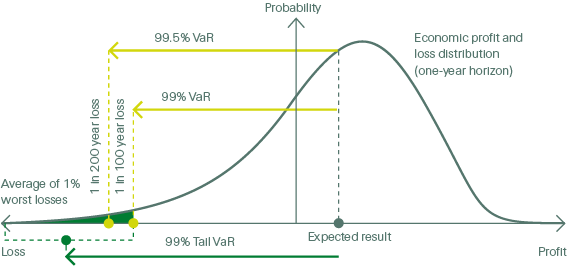
\includegraphics[width=7cm,height=9cm,keepaspectratio]{AAUgraphics/var.png}


\end{frame}

\begin{frame}{Pricing avec Monte Carlo: Value at Risk}{}
  
On peut estimer VaR avec Monte Carlo: $VaR_{99\%}=2$ \\~\\

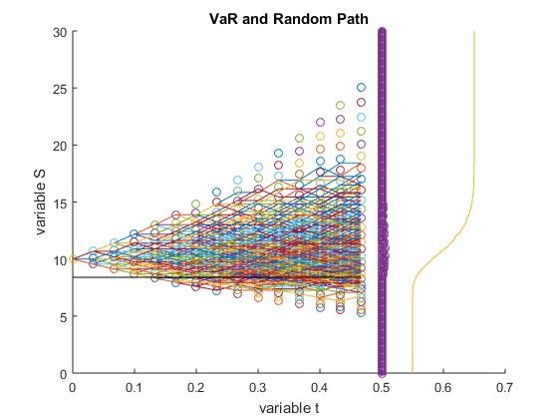
\includegraphics[width=8cm,height=10cm,keepaspectratio]{AAUgraphics/var.jpg}

\end{frame}


\begin{frame}{Pricing avec Monte Carlo: Value at Risk}{}
  
Le percentile 1\% se trouve plus bas $VaR_{99\%} = 5$\\~\\

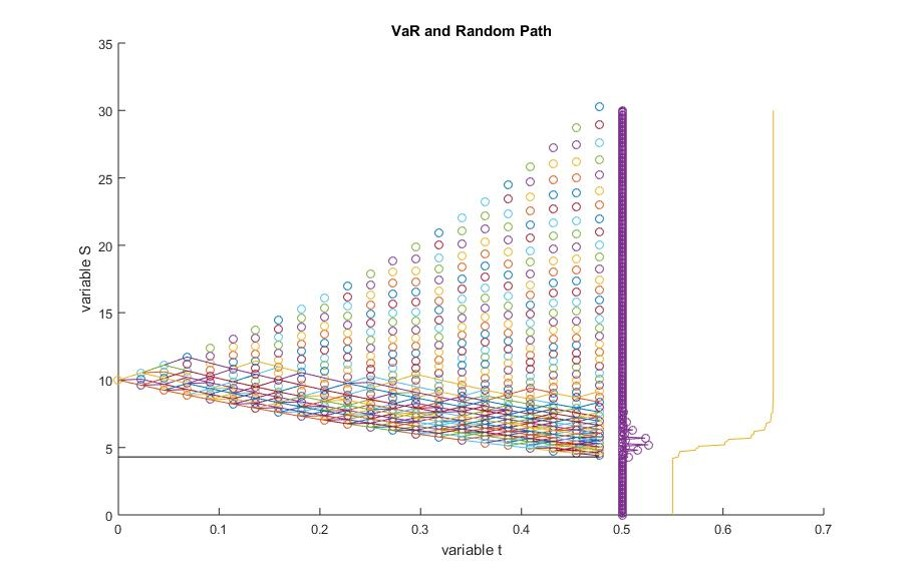
\includegraphics[width=8cm,height=10cm,keepaspectratio]{AAUgraphics/var2.jpg}

\end{frame}








\section{Me contacter}
% contact information
\begin{frame}{Feedback}{Contact Information}
Si vous avez des questions ou des commentaires ou encore si vous trouvez un bug, please n'hésitez pas de me contacter.
  \begin{center}
    \insertauthor\\
    +33783893682
  \end{center}
\end{frame}
%%%%%%%%%%%%%%%%

{\aauwavesbg%
\begin{frame}[plain,noframenumbering]%
  \finalpage{Merci pour votre attention!}
\end{frame}}
%%%%%%%%%%%%%%%%

\end{document}
